\iffalse
\section*{Security Analysis}
\subsection*{A: Risk Identification}
\subsubsection*{Identify Assets}

\textbf{Technologies}
\begin{itemize}
  \item Go, Gin \& Gorm
  \item PostgreSQL
  \item Grafana, Prometheus, Loki \& Promtail
  \item GitHub Actions
  \item Docker
  \item Cypress
  \item Docker Hub
  \item Discord
  \item Vagrant
\end{itemize}

\textbf{Infrastructure}
Our infrastructure is hosted by Digital Ocean. Droplets are VM's running on Digital Ocean's infrastructure. 
\begin{itemize}
  \item Webserver droplet
  \item Database server droplet
  \item Monitoring droplet
\end{itemize}

\subsubsection*{Identify Threat sources}
\begin{itemize}
    \item SSH into droplet
    \item SQL injection
    \item Hacking Digital Ocean account
    \item XSS Attack
    \item Connect to PostgreSQL remotely
    \item Access .env file in webserver container
    \item DDoS (Distributed Denial of Service) attack 
\end{itemize}

\subsubsection*{Construct Risk scenarios}
\begin{itemize}
    \item Attacker knows IP address, computer name for a droplet, and can add their own private key to gain access.
    \item Attacker performs SQL injection on web application to download sensitive user data.
    \item Attacker using brute force or some other way to hack into our Digital Ocean account, giving them access to our whole application.
    \item XSS attack into HTML forms to inject malicious JavaScript
    \item Attacker uses PSQL to access our stuff.
    \item Hacker accesses the .env file inside the webserver docker container (which contains credentials to the database)
    \item Attacker uses a DDOS attack, causing application to shutdown.
\end{itemize}

\subsection*{B: Risk Analysis}
\subsubsection*{Likelihood \& Impact}

\begin{table}[h!]
\begin{tabular}{| l | l | l |}
 \hline
 Name & Likelihood & Impact \\ \hline
 SSH into droplet & Possible &  Major \\ \hline
 SQL injection & Likely &  Major \\ \hline
 Hacking Digital Ocean account & Rare & Severe \\ \hline
 XSS Attack & Likely & Severe \\ \hline
 Connect to PostgreSQL & Rare & Moderate \\ \hline
 Access .env file in webserver & Possible & Severe \\ \hline
 DDOS attack & Likely & Minor \\ \hline
\end{tabular}
\end{table}

Likelihood e.g., Rare, Unlikely, Possible, Likely, Almost Certain
Impact. e.g., Insignificant, Minor, Moderate, Major, Severe

\subsubsection*{Risk Matrix}

\begin{figure}[h!]
\begin{center}
    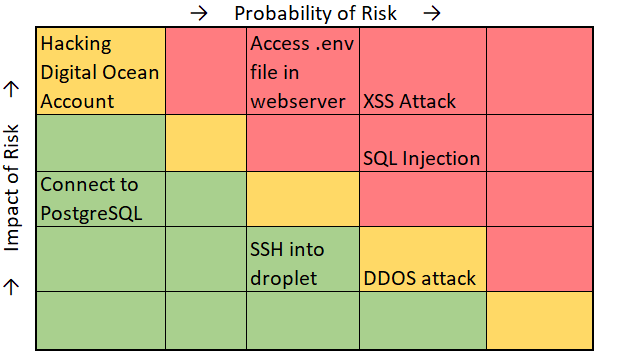
\includegraphics[scale=0.9]{figures/risk assessment.png}
    \caption{Risk Assessment}
  \label{riskmatrix}
\end{center}
\end{figure}

\iffalse
\begin{table}[h]
\begin{center}
\label{tab:mytable} 
\begin{tabular}{| c | c | c | } 
  \hline
  \multicolumn{3}{|c|}{Probability of Risk} \\
  \hline
  \cellcolor{yellow!25}cell1 & \cellcolor{red!25}cell2 & \cellcolor{red!25}cell3 \\ 
  \hline
  \cellcolor{yellow!25}cell1 & \cellcolor{yellow!25}cell5 & \cellcolor{red!25}cell6 \\ 
  \hline
  \cellcolor{green!25}cell7 & \cellcolor{green!25}cell8 & \cellcolor{yellow!25}cell9 \\ 
  \hline
\end{tabular}
\vspace{5mm}
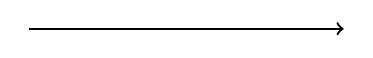
\begin{tikzpicture}
  \draw[->,thick] (0,0) -- (4,0);
\end{tikzpicture}
\end{center}
\caption{Risk Matrix}
\end{table}
\fi

\subsection*{C: Pen-test Your System}
\subsubsection*{Vulnerability scanning}
Used Zaproxy to scan our system for vulnerabilities

\subsubsection*{Vulnerability fixing}
Removed Access .env file in webserver
\fi